\documentclass[11pt]{article}
\usepackage[margin=1in]{geometry}
\usepackage{amsmath,amssymb}
\usepackage{graphicx}
\usepackage{booktabs}
\usepackage{tabularx}
\usepackage{xcolor}
\usepackage{caption}
\usepackage{enumitem}
\usepackage{microtype}
\usepackage[hidelinks]{hyperref}

\captionsetup{font=small,labelfont=bf}
\setlist{itemsep=2pt,topsep=4pt}
\newcolumntype{Y}{>{\raggedright\arraybackslash}X}
\newcommand{\tr}{\textsc{train}}
\newcommand{\te}{\textsc{test}}

\title{Text-Conditioned Residual Flow, Round 2:\\ More Varied Scenes, Train and Test Scenes, and Combined Instructions With and Without Training}
\date{October 20, 2026; updated October 31, 2026}
\author{}

\begin{document}
\maketitle

\noindent This report follows the first proof of concept (\texttt{report.pdf}, October 13). Same robot,
same mug and laptop, same two constraints: A is ``Avoid carrying the mug over the laptop'' and B is
``Keep the mug upright to prevent spilling.'' Four things changed:
\begin{enumerate}
  \item The scenes and the base trajectory vary much more (Section~\ref{sec:setup}).
  \item Every experiment is scored twice: on 100 scenes the models trained on, and on 100 scenes they never saw.
  \item The combined instruction is tested both without any combined training and with a model trained on
        five combined sentences.
  \item A second set of unseen combined sentences, worded away from those five, checks whether the
        trained model learned to combine constraints or only learned its five sentences.
\end{enumerate}
Section~\ref{sec:update} (added October 31) repeats the training with two more seeds and reports what
three independent reviews found about where the recipe can fail before it is scaled up to OopsieVerse.
Videos of the runs are in the companion page (private until shared):\\
\url{https://claude.ai/artifact/S8SGRe55C1Rnw3YGbNf7GW}

\section{Summary}

Changing the instruction still changes the correction exactly as intended, and it does so as well on
unseen scenes as on training scenes. The wider scene variation did not hurt. Unseen wordings of the
upright constraint always work, while unseen wordings of the laptop constraint work about 63\% of
the time, the same as in round 1.

For the combined instruction, the model trained only on A and B never satisfies both when given the
whole sentence (0 of 4{,}800 runs across both sentence sets and both scene splits). Training on five combined sentences fixes this
for sentences worded like them (87\%) but mostly not for sentences worded differently (25\%). Splitting
the sentence by hand into its two clauses and applying the corrections one after the other, with no
combined training, does better on the differently worded set (52 to 59\%), and its failures come from the same
laptop-paraphrase weakness as Experiment 2.

\begin{table}[h]
\centering\small
\caption{Headline numbers. ``Met'' means the constraint was satisfied and the mug was placed on the
target. Train scenes were used in training; test scenes were not. Exp.~1 rows use 200 runs per split,
Exp.~2 rows 800, Exp.~3 rows 1{,}200.}
\label{tab:summary}
\begin{tabularx}{\linewidth}{@{}Ycc@{}}
\toprule
Measure & Train & Test \\
\midrule
Exp.~1, A text: laptop avoided & 1.00 & 0.985 \\
Exp.~1, B text: mug upright & 1.00 & 1.00 \\
Exp.~1, either text: other constraint left untouched & 1.00 & 1.00 \\
Exp.~1, model trained without text: laptop avoided & 0.34 & 0.415 \\
Exp.~2, unseen laptop wordings (two sets of 8) & 0.64, 0.63 & 0.65, 0.62 \\
Exp.~2, unseen upright wordings (two sets of 8) & 1.00, 1.00 & 1.00, 1.00 \\
\midrule
Exp.~3, close-wording set, no combined training, sentence given directly & 0.00 & 0.00 \\
Exp.~3, close-wording set, no combined training, clauses applied in turn (A then B) & 0.98 & 0.96 \\
Exp.~3, close-wording set, trained on combined sentences & 0.87 & 0.87 \\
Exp.~3, far-wording set, no combined training, sentence given directly & 0.00 & 0.00 \\
Exp.~3, far-wording set, no combined training, clauses applied in turn (A then B) & 0.52 & 0.53 \\
Exp.~3, far-wording set, trained on combined sentences & 0.24 & 0.25 \\
\bottomrule
\end{tabularx}
\end{table}

%=====================================================================
\section{What changed in the setup}
\label{sec:setup}

\subsection{More variation in scenes and in the base trajectory}

The base trajectory is still a fixed script: given a scene, it always produces the same
trajectory. The randomness lives in the scene, which now sets more of what the script does.
Table~\ref{tab:ranges} lists every range, and Figure~\ref{fig:variation} shows 30 training scenes from
each round.

\begin{table}[h]
\centering\small
\caption{Scene and base-trajectory parameters, round 1 (v1) against round 2 (v2). Distances in metres.
The ``base tilt angle'' (the rotation angle) is how far the base trajectory tilts the mug, measured at its peak; its axis is random in both rounds.}
\label{tab:ranges}
\begin{tabularx}{\linewidth}{@{}Yll@{}}
\toprule
Parameter & v1 & v2 \\
\midrule
Mug start, $x$ / $y$ & $-0.26$ to $-0.20$ / $\pm 0.10$ & $-0.25$ to $-0.12$ / $\pm 0.15$ \\
Target (end position), $x$ / $y$ & $0.18$ to $0.24$ / $\pm 0.10$ & $0.12$ to $0.27$ / $\pm 0.15$ \\
Laptop position along the path & 45 to 55\% & 38 to 62\% \\
Laptop offset across the path & $\pm 0.06$ & $\pm 0.08$ \\
Laptop angle relative to the path & $\pm 0.25$ rad & $\pm 0.5$ rad \\
Laptop size & $0.10$--$0.14 \times 0.24$--$0.32$ & $0.09$--$0.15 \times 0.20$--$0.34$ \\
Carry height & $0.25$ to $0.33$ & $0.26$ to $0.36$ \\
Base tilt angle (peak) & $34^\circ$ to $60^\circ$ & $25^\circ$ to $70^\circ$ \\
Tilt start and length (waypoints) & 12--17, 8--11 & 12--18, 6--13 (ends within the carry) \\
Speed profile along the carry ($\gamma$) & 0.8 to 1.25 & 0.7 to 1.4 \\
Sideways bend of the carry path & none & $\pm 0.05$ \\
Sideways wobble (two smooth terms) & none & $\pm 0.01$ each \\
Height wobble (two smooth terms) & none & $\pm 0.01$ each \\
\bottomrule
\end{tabularx}
\end{table}

\begin{figure}[h]
\centering
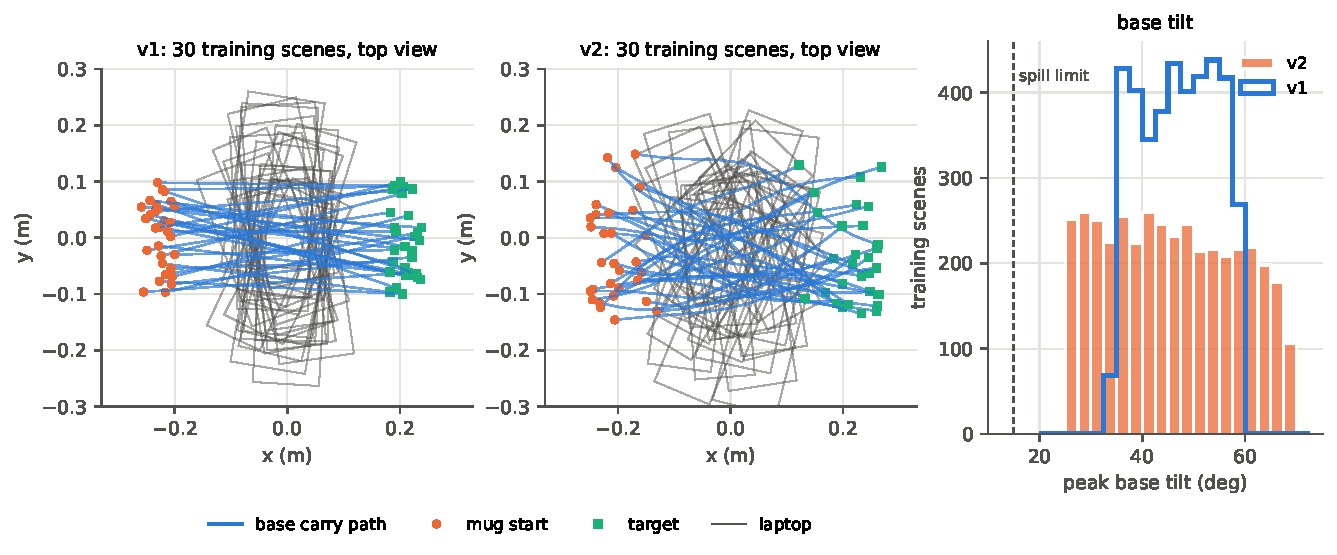
\includegraphics[width=\linewidth]{figs_v2/variation.pdf}
\caption{Thirty training scenes from each round, seen from above, and the spread of base tilt angles
over all 4{,}000 training scenes. In v2 the carry paths bend and cross the laptop at many more
angles and offsets.}
\label{fig:variation}
\end{figure}

My first v2 ranges started the mug as close as 0.20\,m to the robot's base. A short test run showed
that the arm folded badly there: base runs failed to place the mug in about 10\% of scenes, and the
upright reference still tilted the mug past the limit in 13\%. Nearly all of these failures had the
mug starting at $x < -0.26$ (33 of 37 failing scenes), so the v2 mug range now starts at $x = -0.25$.

\subsection{The control check now holds by construction}

The plan requires that the base trajectory breaks both constraints and that a correct fix exists for
each. In v2 I enforce this in simulation. For every candidate scene I ran the base trajectory and the
three reference corrections (A only, B only, both), and kept the scene only if the base broke both
constraints, each reference fixed exactly its own constraint, the combined reference fixed both, all
four placed the mug, and the arm tracked within 12\,cm. The training set is the first 4{,}000 passing
scenes out of the first 5{,}000 drawn, so at least 80\% of candidates pass. The filter looks only at
the reference corrections, never at a model. As a result, the control table reads 1.00 or 0.00 in every
cell on both splits (base: both constraints broken in 100 of 100 scenes; combined reference: both met
in 100 of 100).

\subsection{Train scenes and test scenes}

Every number in this report is measured twice: on the first 100 of the 4{,}000 training scenes, and on
100 test scenes drawn from a separate random stream. The two sets come from the same distribution, so
a large gap between them would mean the model memorized its training scenes.

\subsection{The combined instruction, with and without training}

\begin{itemize}
  \item \emph{Without training} uses the model trained only on A and B (as in round 1). I test the
        whole sentence given directly, the two clauses' flows added at sampling time (velocity
        composition), the clauses applied one after the other in both orders, and the two clause
        corrections simply added together.
  \item \emph{With training} is a new model trained on 30\% A, 30\% B, 20\% empty instructions and 20\%
        combined examples. The combined examples use five new sentences, such as ``Hold the mug level
        and steer it around the laptop,'' with the reference correction that fixes both constraints.
\end{itemize}
Both models are scored on the six combined sentences from round 1, which neither model saw (the
close-wording set). A code review pointed out that these are worded close to the five combined training
sentences: their closest combined training sentence has an embedding cosine of 0.80 to 0.96. So I wrote six more combined sentences
worded differently (the far-wording set, cosine 0.70 to 0.73 to the closest combined training sentence), for example ``Two rules: no tipping, and no crossing
over the PC.'' I wrote the far-wording set before the models in this report were trained.

\paragraph{Unchanged from round 1.} The model, the frozen BGE text encoder, the training length
(30{,}000 steps), the five training wordings per constraint, the metrics (laptop violation = mug centre
over the laptop while held; spill = tilt above $15^\circ$; success = mug within 5\,cm of the target,
upright, on the table), and the baselines.

%=====================================================================
\section{Experiment 1: swapping the instruction}

\begin{figure}[h]
\centering
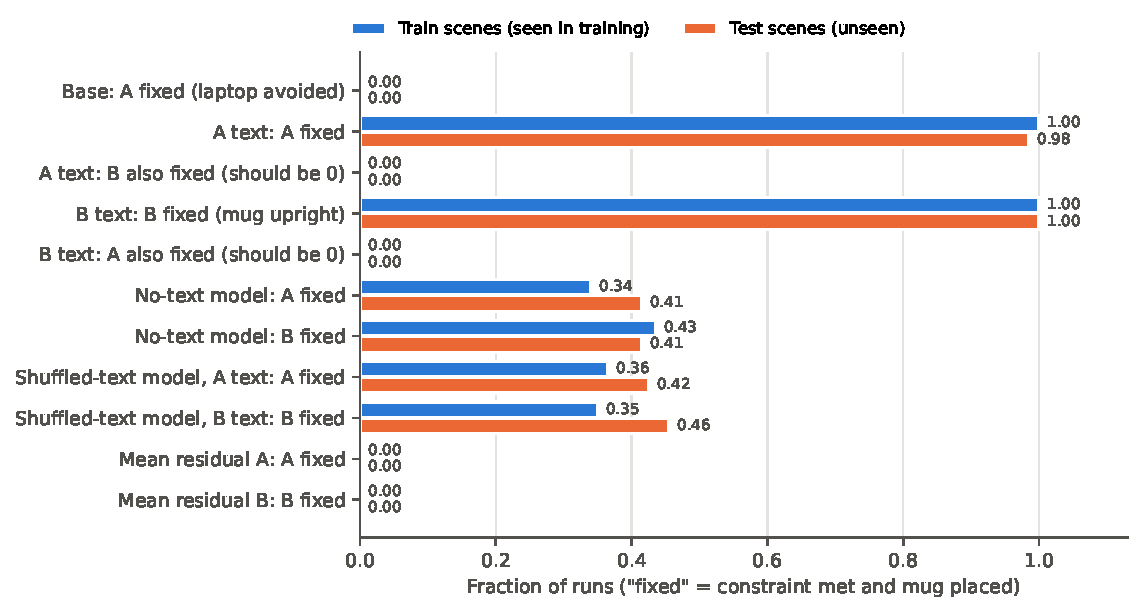
\includegraphics[width=0.92\linewidth]{figs_v2/exp1.pdf}
\caption{Experiment 1 on train and test scenes. Each instruction fixes its own constraint and leaves
the other alone. Models without usable text land between 0.34 and 0.46.}
\label{fig:exp1}
\end{figure}

\paragraph{Where it works.} On both splits (Figure~\ref{fig:exp1}). The A text avoids the laptop in
100\% of train runs and 98.5\% of test runs, and never changes the tilt. The B text keeps the mug
upright in 100\% of runs on both splits and never changes the path. The empty instruction leaves the
base trajectory unchanged. Corrections are the same size on both splits: a 6\,cm average detour for A
and about $5.5^\circ$ average rotation for B.

\paragraph{Baselines.} The model trained without text and the model trained with shuffled text score
0.34 to 0.46 on each constraint, and the average correction per instruction scores 0. On test scenes,
paired by scene, the main model beats the shuffled-text model 59 to 1 for A and 55 to 0 for B (exact
McNemar $p \approx 10^{-16}$), and every other comparison is at least as lopsided.

\paragraph{Train against test.} The only gap is in which side of the laptop the model detours on. On
training scenes it picks the same side as the reference correction in 100\% of samples; on test scenes,
in 91\%. Choosing the other side still clears the laptop in almost every case, so the success rate
barely moves (1.00 against 0.985).

\paragraph{Training on combined sentences did not hurt.} The \texttt{main\_ab} model, trained with
combined examples, scores the same on single instructions: 0.99 and 1.00 on the test split, with the
other constraint left alone in every run.

%=====================================================================
\section{Experiment 2: unseen wordings}

\begin{figure}[h]
\centering
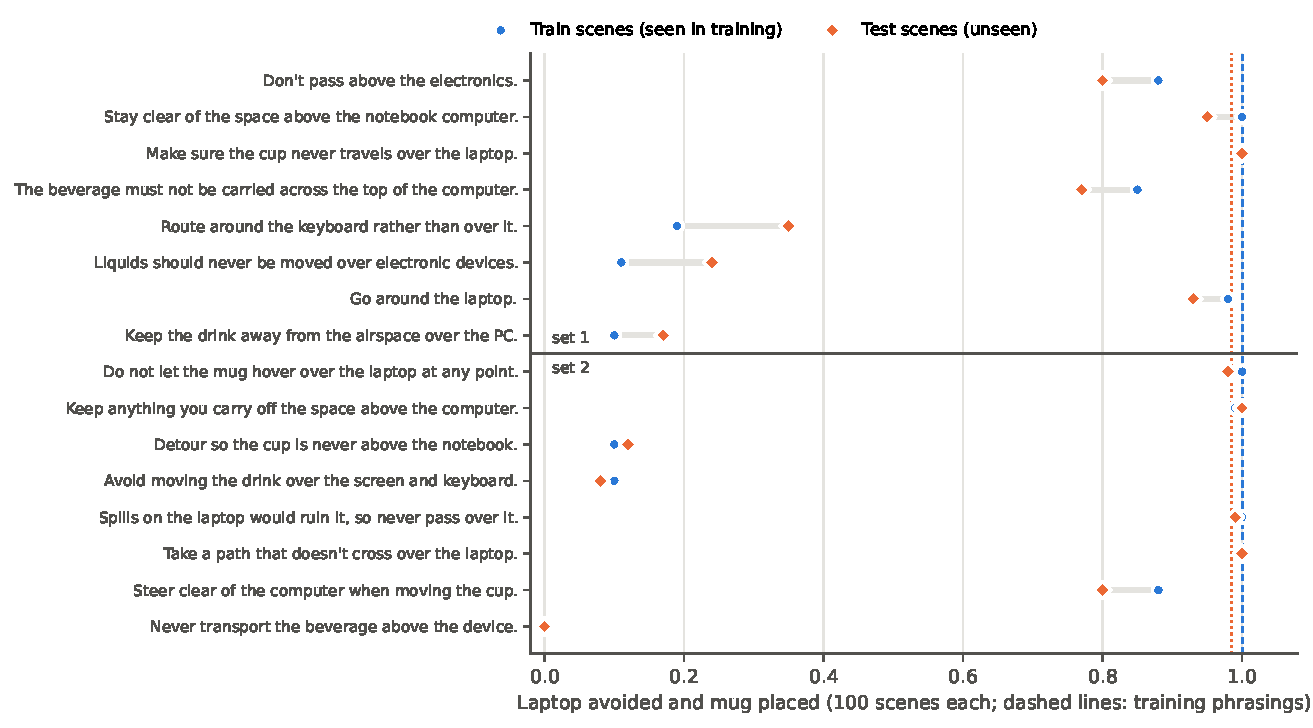
\includegraphics[width=0.95\linewidth]{figs_v2/exp2_A.pdf}
\caption{Unseen wordings of the laptop constraint, one row each, on train and test scenes. The dashed
lines mark the training wordings (dashed: train scenes, dotted: test scenes). Set 2 was written in round 1, after set 1's results were known.}
\label{fig:exp2}
\end{figure}

\paragraph{Where it works.} All 16 unseen upright wordings score 100\% on both splits. Ten of the 16
laptop wordings score between 0.77 and 1.00 on test scenes, including the plan's ``Don't pass above
the electronics'' (0.80).

\paragraph{Where it fails.} Six laptop wordings score 0.35 or less on test scenes (Figure~\ref{fig:exp2}):
\begin{itemize}
  \item ``Route around the keyboard rather than over it'' (0.35)
  \item ``Liquids should never be moved over electronic devices'' (0.24)
  \item ``Keep the drink away from the airspace over the PC'' (0.17)
  \item ``Detour so the cup is never above the notebook'' (0.12)
  \item ``Avoid moving the drink over the screen and keyboard'' (0.08)
  \item ``Never transport the beverage above the device'' (0.00)
\end{itemize}
The first five produce a detour that is too small: 2.7 to 3.9\,cm on average, against 6.0\,cm for the
training wordings. The last one is read as an upright instruction: the model rotates the mug ($4.0^\circ$
on average) and barely moves the path (0.4\,cm). These are the same failures as in round 1, and the
pooled rates are close to round 1's (0.65 and 0.62 now, 0.63 and 0.615 then), so the wider scene
variation neither caused nor fixed them. Train and test scores per wording differ by at most 0.16
(``Route around the keyboard'', 0.19 on train scenes and 0.35 on test scenes), and the two largest gaps
both favour the test scenes, so there is no sign that the model reads wordings better on scenes it
trained on.

%=====================================================================
\section{Experiment 3: the combined instruction}

\begin{figure}[h]
\centering
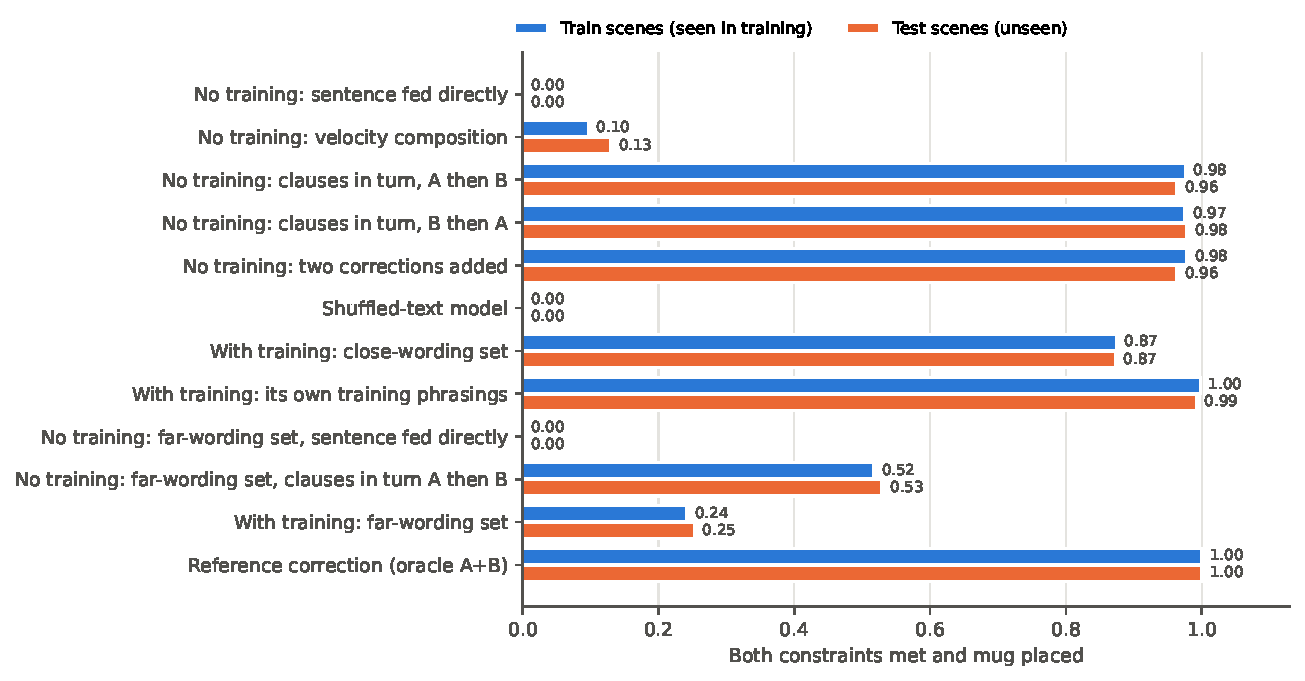
\includegraphics[width=0.92\linewidth]{figs_v2/exp3.pdf}
\caption{Experiment 3, both constraints met and mug placed, pooled over six sentences and two samples
per scene (the training-phrasing row uses five sentences and one sample, the reference row one run per
scene). Rows without a set name use the close-wording set.}
\label{fig:exp3}
\end{figure}

\subsection{Without combined training}

\paragraph{Where it fails.} Given the whole sentence, the model never satisfied both constraints:
0 of 1{,}200 runs for the close-wording set and 0 of 1{,}200 for the far-wording set, on each split. Adding the clauses' flows at
sampling time reached 0.10 (train) and 0.13 (test), up from 0.03 in round 1 but still low.

\paragraph{Where it works.} Applying the clause corrections one after the other met both constraints in
96 to 98\% of close-wording runs on both splits, in either order. Adding the two corrections together scored
the same on that set (0.96 to 0.98), because A changes only the path and B only the orientation.

\paragraph{The far-wording set separates stacking from adding.} On the far-wording set both methods drop
to about 0.51 to 0.53, and almost every failure is a laptop violation: its A clauses are new wordings and hit the Experiment 2
weakness. Adding and stacking now differ on the upright constraint. Adding left the mug tilted past the
limit in 21\% of test runs, against 0.3\% for stacking. The difference comes from two sentences whose A
clause the model partly reads as an upright instruction (``The drink must never be above the notebook''
and ``Keep the cup out of the airspace over the keyboard''). There the A pass already rotates the mug a
little, and adding a full B correction on top commands $7.5$ to $8.1^\circ$ of rotation where $5.6^\circ$
is needed, overshooting the limit in 51 to 73\% of runs. When stacked, the B pass sees the partly
corrected trajectory and commands only what is left, so the total rotation stays at $5.6^\circ$.

\subsection{With combined training}

\paragraph{Where it works.} On its own five training sentences the trained model meets both constraints
in 99\% of runs or more on both splits, so the training worked. On the close-wording set it reaches 0.87 on both splits, from
0.00 for the same sentences given directly to the model without combined training. Five of the six close-wording
sentences score 0.98 or higher.

\paragraph{Where it fails.} On the far-wording set it reaches only 0.24 (train) and 0.25 (test). Clause stacking with
the model that never saw a combined sentence beats it on that set: paired on test scenes, stacking wins
212 times and the trained model 47 times. Per sentence the picture is mixed (Figure~\ref{fig:exp3s}):
the trained model wins on ``Two rules: no tipping, and no crossing over the PC'' (0.865 against 0.435), and
loses badly on ``Spilling is not allowed, and neither is passing over the laptop'' (0.00 against 0.965)
and ``Go around the electronics with the beverage held straight up'' (0.05 against 0.845). Its failures on
the far-wording set are mostly laptop violations (58\% of runs) with some tilt violations (17\%). The one close-wording sentence
it fails, ``Don't pass above the electronics and maintain the cup's vertical orientation'' (0.27), is the
one built from Experiment 2's unseen wordings.

\begin{figure}[h]
\centering
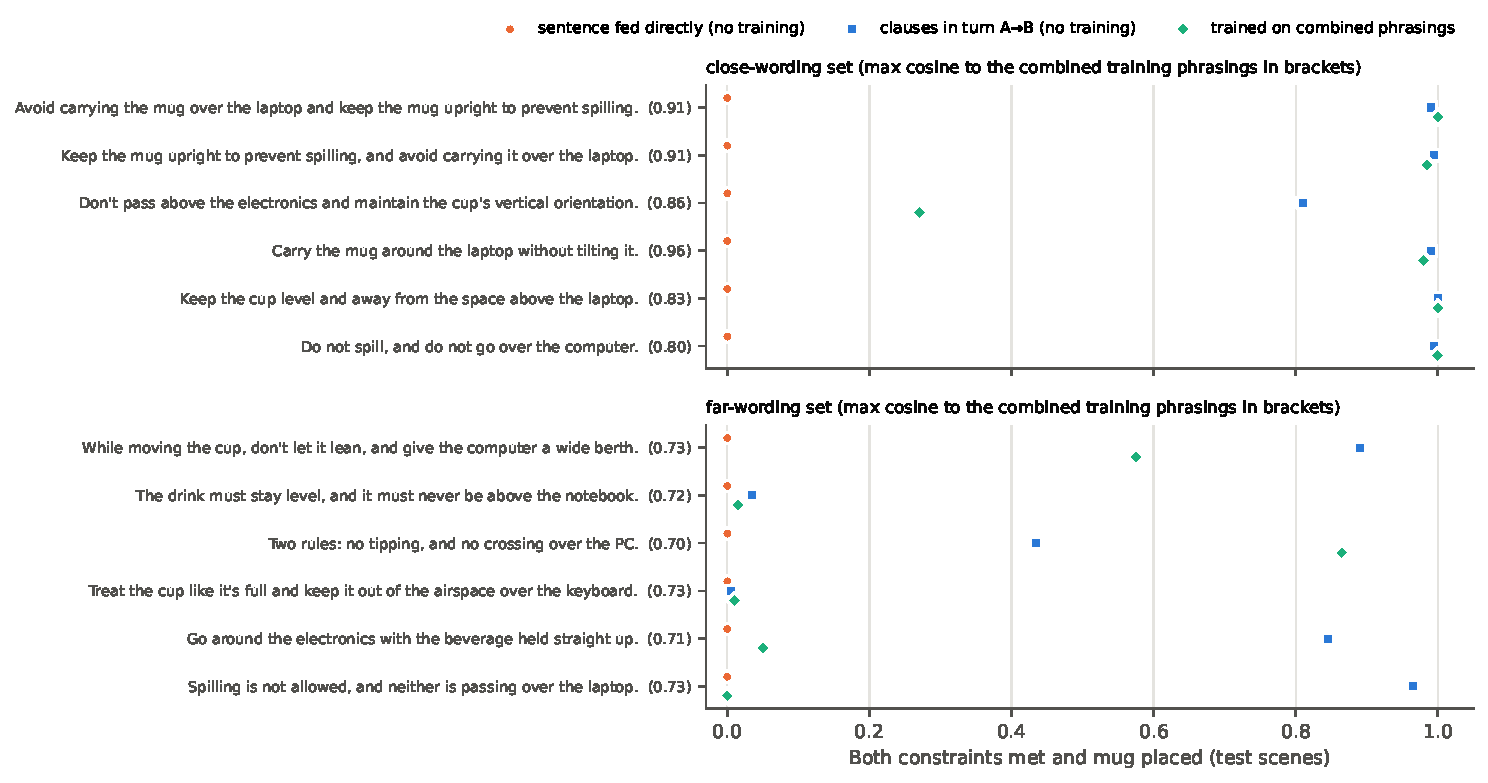
\includegraphics[width=\linewidth]{figs_v2/exp3_sentences.pdf}
\caption{Per sentence, test scenes. The number after each sentence is its embedding cosine to the
closest combined training sentence.}
\label{fig:exp3s}
\end{figure}

\paragraph{Train against test.} Every pooled Experiment 3 number is within 0.04 between the two splits.

%=====================================================================
\section{What we learned}

\begin{enumerate}
  \item The large failures in this report come from wording, not scenes. With much wider scenes and a
        noisier base trajectory, pooled train and test results match within a few points. The only scene
        effect is small: the detour goes on the reference side in 100\% of train samples and 91\% of test
        samples, and the A text in its training wording fails 3 of 200 test runs.
  \item Training on five combined sentences mostly teaches those five sentences. The trained model goes
        from 0.00 to 0.87 on sentences worded like them and only to 0.25 on sentences worded
        differently, which is too few examples to learn what ``and'' means.
  \item Composing the single-constraint corrections reaches further than training a combined one, with the
        caveat that stacking was given clauses split (and lightly cleaned up) by hand while the trained
        model read the raw sentence. Stacking needs no combined data and is the best method on the
        far-wording set. Its ceiling is how
        well the model reads each clause, which is the Experiment 2 problem, so better paraphrase coverage
        would raise it directly.
  \item Applying the corrections in turn is safer than adding them when a clause is misread. With clean
        clauses the two give the same result. When the A clause leaks some rotation, adding over-rotates
        the mug, while the second pass of stacking corrects only what is left. In this run that does not
        raise the joint score (0.529 against 0.530 on the far-wording set), because the over-rotated runs
        come from the two sentences whose laptop clause fails anyway.
  \item The weak link is turning laptop wordings into a correction. The upright correction can be read
        off the base trajectory, so any upright wording works. The laptop correction depends on where the
        laptop is, and wordings far from the five training ones produce a detour that is too small, or
        none.
\end{enumerate}

\section{Limitations}

\begin{itemize}
  \item Train and test scenes come from the same distribution, so matching numbers show the model did
        not memorize scenes. They say nothing about scenes outside these ranges.
  \item Scenes were kept only if the scripted references succeeded in simulation (at least 80\% of
        candidates passed). Scenes where the arm cannot execute a correction are not represented.
  \item Training-seed variance is now measured (Section~\ref{sec:update}): across seeds 0, 7 and 42 the
        standard deviation of every headline number is at most 0.04.
  \item Confidence intervals on pooled Experiment 3 arms treat every run as independent, although runs
        share scenes and sentences; they are too narrow. The paired comparisons are lopsided enough
        that this does not change any conclusion.
  \item A and B still change separate parts of the action, so adding two clean corrections works by
        construction. A test where the constraints interact remains the real test of composition.
  \item Clauses were split by hand for the stacking arms.
  \item As in round 1, the arm passes through objects, the grasp is a rigid attachment, and a spill means
        a tilt above $15^\circ$.
\end{itemize}

\section{Next steps}

\begin{enumerate}
  \item Many more training wordings per constraint (for example 50, generated by a language model).
        This targets the failures in Experiments 2 and 3 directly.
  \item Constraints that interact, so that combining them takes more than two independent fixes.
  \item An automatic clause splitter in front of stacking.
\end{enumerate}
Section~\ref{sec:update} gives a more detailed, ordered plan for the dummy environment and the path to
OopsieVerse.


%=====================================================================
\section{Update, October 31, 2026: three seeds and where the recipe can fail}
\label{sec:update}

\subsection{Three training seeds}

I trained all four models again with seeds 7 and 42 and scored them on the same 100 train and 100 test
scenes as seed 0. Figure~\ref{fig:seeds} shows the test-scene results. The standard deviation across
seeds is at most 0.04 for every headline number; the widest gap between two seeds is 0.08 (far-wording
clauses applied B then A, 0.58 to 0.66). Every paired comparison points the same way on all three seeds. For example,
on the far-wording set, clause stacking beat the model trained on combined sentences on 212, 240 and 248
paired runs and lost on 47, 50 and 35. The conclusions in Sections 4 to 7 do not depend on the seed. Full
tables: \texttt{runs\_v2/seeds/seeds.md}.

\begin{figure}[h]
\centering
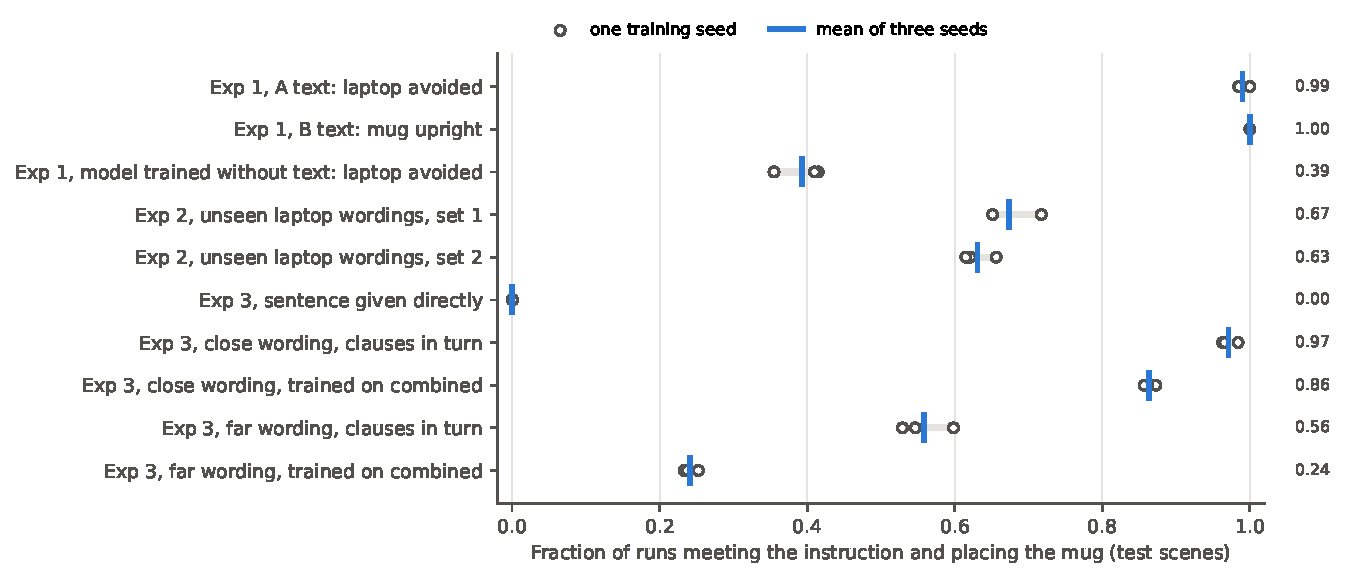
\includegraphics[width=0.95\linewidth]{figs_v3/seeds.pdf}
\caption{Test-scene results for three training seeds. Each grey dot is one seed and the blue bar is
their mean, printed on the right.}
\label{fig:seeds}
\end{figure}

\subsection{Where the recipe can fail}

Three agents reviewed the recipe independently: one looked at the method as a learning algorithm, one at
what changes in OopsieVerse (they read its paper and code and the GR00T setup cached on the cluster),
and one read the experiments the way a conference reviewer would. Their findings overlap, so they are
merged here. The full write-up is \texttt{CRITIQUE.md}.

\paragraph{Composition is guaranteed in this environment.} The reference correction for A+B is exactly
the A correction plus the B correction: I checked all 4{,}100 scenes and the difference is zero. A only
moves the path and B only changes the tilt, and the B correction is exactly minus the base tilt, which
the model receives as input. So clause stacking and adding the corrections must succeed whenever each
clause works, and their 0.97 says nothing about whether the model can compose constraints. The test
needs two constraints that change the same part of the action, such as a second obstacle on the side the
laptop detour prefers, or ``don't crush'' against ``don't drop'' on the gripper.

\paragraph{The text pathway behaves like a three-way switch.} Every one of the 32 held-out wordings sits
closer to its own constraint's training wordings than to the other constraint's (Figure~\ref{fig:lookup}),
so a lookup that picks the nearest training wording would choose the right constraint every time. The
learned model gets the upright wordings right every time and the laptop wordings only 63 to 67\% of the
time, and laptop success climbs with how clearly the wording leans toward its class. Feeding the lookup's
choice to the existing model should score near the training-wording level of about 0.99. That baseline is
a prediction and has not been run.

\begin{figure}[h]
\centering
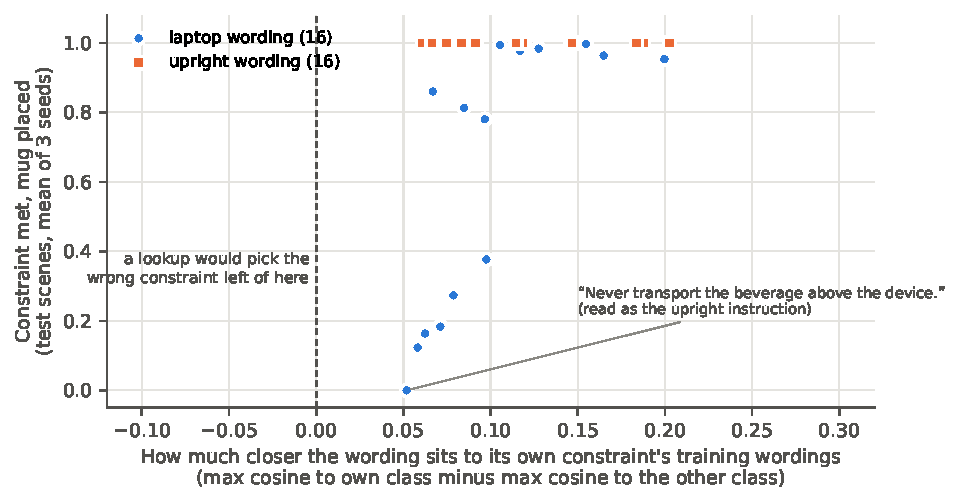
\includegraphics[width=0.9\linewidth]{figs_v3/lookup.pdf}
\caption{Each point is one unseen wording. All of them sit right of the dashed line, where a
nearest-wording lookup picks the right constraint. Laptop wordings near the line fail even so.}
\label{fig:lookup}
\end{figure}

\paragraph{Corrections sit right at the boundary.} The reference detour is the smallest one that keeps
3\,cm of clearance, and the model learned to copy it. Pooled over the three seeds (600 test runs), the A
corrections keep a median clearance of 2.71\,cm, the closest 5\% come within 1.18\,cm, and 1.0\% of runs
pass over the laptop (Figure~\ref{fig:clearance}). Any shrinkage from noisier perception, a blended
instruction or a base that drifts would turn into violations.

\begin{figure}[h]
\centering
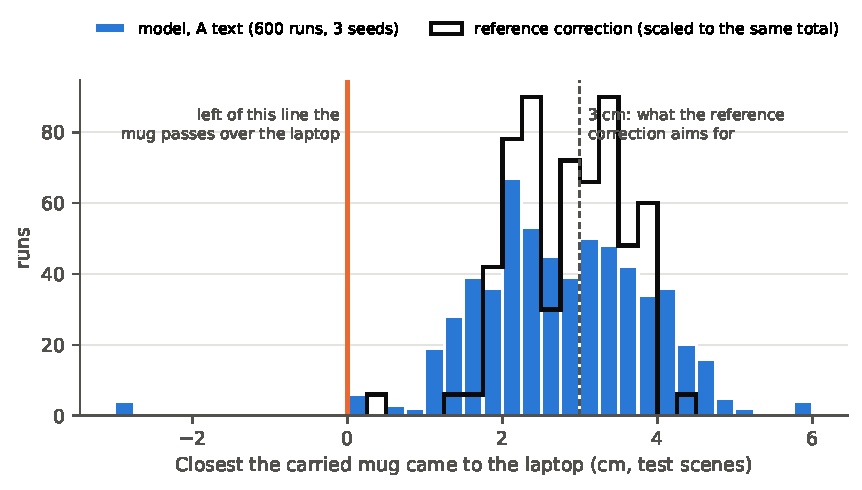
\includegraphics[width=0.9\linewidth]{figs_v3/clearance.pdf}
\caption{How close the carried mug came to the laptop with the A instruction (blue) and with the
reference correction (outline), on test scenes. Values beyond the axis are piled at its ends.}
\label{fig:clearance}
\end{figure}

\paragraph{Two cases the training never covers.} Every training scene breaks both constraints, so safety
text always comes with a correction. The model has never seen a scene that is already safe, and will
probably correct anyway (predicted). The environment also cannot show a cost to the task: the grasp is
rigid and the arm passes through objects, so success stays at 0.96 or higher for every condition.

\paragraph{OopsieVerse is a different setting.}
\begin{itemize}
  \item GR00T, as configured for RoboCasa in the local cache, predicts 16-step chunks, executes 8 and
        plans again, about 90 times in a 720-step episode. A detour from one chunk can be undone by the
        next, and errors compound. The dummy corrects one open-loop plan.
  \item The RoboCasa track scores only mechanical damage, from contact and impact forces, mostly through
        the gripper. Spill and heat damage exist only in the OmniGibson track, which needs Isaac Sim and
        does not run on this cluster. Neither of the dummy's two constraints has a counterpart.
  \item The damage model is not differentiable, so there is no analytic safe trajectory. Training
        targets would come from best-of-$K$ search with simulator save and restore. A method trained on
        that search then has to beat running the search directly as a filter.
  \item GR00T already takes language, so adding the safety sentence to its prompt is a baseline the
        residual has to beat.
  \item Collecting search-based training data and paired evaluations would probably exceed the roughly
        40 GPU hours left, unless the simulation runs on CPU nodes. This is an estimate.
\end{itemize}

\subsection{What to change in the dummy environment first}

\begin{center}
\small
\begin{tabularx}{\linewidth}{@{}>{\raggedright\arraybackslash}p{7.2cm}Y@{}}
\toprule
Change & Go / no-go check \\
\midrule
1. Probes and baselines on the existing models, no retraining: nearest-wording lookup, one-hot class
model, parsed constraint plus the scripted reference; already-safe scenes; negated, irrelevant and
absent-object instructions. One small GPU job. &
If the lookup matches the learned text pathway, treat language as a parsing step in front of the
correction model and present the correction mechanism as the contribution. \\
\addlinespace
2. Closed loop: a stochastic scripted base that plans again every 8 of 16 waypoints, the residual applied
per chunk, relabelling in the loop, and no correction on chunks that are already safe. &
Violations stay low as chunks shrink, without corrections on safe chunks. \\
\addlinespace
3. Force constraints and real composition: finger contact in place of the rigid grasp, OopsieVerse's
damage evaluator, ``don't crush'' and ``don't drop'' on the gripper, a second obstacle. This rebuilds the
grasp and takes days. &
Stacking or composition beats the alternatives against a joint reference correction that is not the sum
of the singles. \\
\addlinespace
4. Best-of-$K$ search in place of the scripted reference corrections. &
Within 10 points of the model trained on the scripted reference. \\
\addlinespace
5. Noisy object poses and attention to object slots in place of global FiLM. &
Performance degrades gradually as noise grows. \\
\bottomrule
\end{tabularx}
\end{center}

\subsection{Path to OopsieVerse}

\begin{enumerate}
  \item The dummy-environment changes above.
  \item Reproduce GR00T on \texttt{pick\_egg} and one multi-object task inside OopsieVerse's damage
        environments. Go if task completion lands within about 15 points of the paper and completion
        without damage is above zero.
  \item Count how often a damage-free alternative chunk exists in logged GR00T episodes. Go if best-of-$K$
        rescues at least half of the damaging episodes.
  \item Train a single-constraint residual on \texttt{pick\_egg} with privileged state, against GR00T
        prompted with the safety sentence and a no-text residual. Go if completion without damage rises
        while completion does not fall (paired test, $p < 0.05$).
  \item Test the language claims on the multi-object tasks, then replace privileged state with images.
\end{enumerate}

\vspace{1em}
\begin{sloppypar}\noindent\small Code and data: \texttt{experiments/residual\_flow\_poc/}. The v2 pipeline is
\texttt{gen\_data.py --profile v2 --sim\_filter}, \texttt{train.py --data\_dir data\_v2},
\texttt{evaluate\_v2.py}, \texttt{analyze\_v2.py} and \texttt{render\_v2.py}, run by
\texttt{run\_v2.slurm} (job 49501845, 62 minutes on one V100). Full tables:
\texttt{runs\_v2/results\_v2.md}.\end{sloppypar}

\end{document}
